\documentclass[11pt]{article}
\usepackage{techcon13_LaTeX_style}
\usepackage{subfig}
\begin{document}

% NOTE: Do not change any of the LaTeX commands in this file unless
%       you really know what you are doing.  Further, any changes you
%       make must meet the Tech Con '13 abstract guidelines



%Service Choreography Simulator with QoS compisition
  %QoS Service choreography support through Simulator
  %QoS support in service choreography through a simulator engine
\tctitle{
  A simulator for QoS Service choreography support
}

\tcauthor{
Alfonso Phocco Diaz, Daniel Batista,  Dejan Milojicic
}

\tcbusinessgroup{
University of S\~{a}o Paulo, Brazil\\
HP Labs Palo Alto, USA
}

\tcemail{
\{alfonso7, batista\}@ime.usp.br; dejan.milojicic@hp.com
}

\tcabstract{

 Service choreography allows the composition of services in a collaborative way, because of global description and descentralized 
coordination using interactions P2P among participants. However, since   infraestructures and implementations aren't mature enough
 to enact choreographies, then to evaluate and analyse how the environment affects the QoS requirements and composition behavior 
into a choreography is a difficult task. To be able to do so, we propose to develop a choreography simulator in order to simulate 
enacting of choreographies.  

 In this work, we also  propose a QoS model for implementing  on the choreography simulator taking  into account QoS composition, infraestructure
 and environment aspects.  Furthermore, we adopted a choreography scenario about Content Delivery Network (CDN) providing
 streaming multimedia objects.

}

\section*{Problem statement}

Among the various methods to compose services, Web services choreography is an efficient way to implement inter-organizational business
 processes, as the participants' business interactions are mutually independent (autonomous and heterogeneous) \cite{Telang2011}. A service
 choreography is a description of peer to peer interactions among existing services, i.e., in this model there isn't the role of 
 a central controller. The various services communicate with each other similarly to what occurs in a P2P applications \cite{Barker2009}. 

Due to the increasing number of devices joining the Internet,
a centralized approach like an orchestration may not be sufficiently
scalable in terms of network bandwidth to deal with the
ever escalating number of devices and services that may be
available. Within such a scenario, a decentralized approach,
like choreographies, may turn out to be more capable of
dealing with such high complexity (trecho do artigo do Felipe e Eduardo, d� para tirar ele).

 During the enactment of  services choreographies, the state of network elements (devices and links) plays a fundamental role. There must be guarantees 
 of Quality of Service - QoS so that there are advantages of using a decentralized business model. A common method to define
 guarantees between a service provider and a client (which may also be a service) is by means of a Service Level Agreement - SLA. After
 the choreography be specified,  constraints of QoS between each participant must be defined through SLAs \cite{Rosenberg2007}. To meet the SLA 
 agreements there must be some mechanism for management at runtime. This mechanism must involve monitoring, control and  
 decisions against violations or degradation of service quality. All the concern about guarantee of the QoS requirements of participants comes 
 from the fact that the QoS of composite service, represented by the choreography, depends directly on the QoS of the separate services.

% To reduce the number of SLA violations and the corrective measures to fulfill the QoS requirements during the enactment of choreographies, 
% the detection of non-functional failures in early stages of the development of the choreography can be employed.

Currently, to implement and enact a real service choreography is still difficult because of immature technology support, especially
by lack of Choreography aware engine execution~\cite{Kopp2010}. Then, performance evaluations, QoS measurements, QoS requirements
 establishment, monitoring, and so on, aren't very developed.

%And in choreography  non-functional failures (or undesirables properties)  are communication and network errors such as high latency and low bandwidth are important
%aspects.



\section*{Our solution}

The objective of our work is to develop a simulator in order to enact services choreographies  and enable QoS support taking into account 
the infrastructure and  environment aspects. For achieve this, we  use a QoS model about  service, message and communication attributes involved 
in a service choreography.  Moreover, to attest the efficacy of our simulator we adopt a choreography scenario about Content Delivery Network (CDN) providing
 streaming multimedia objects~\cite{Buccafurri2008a}. %%and we show some experimental results, or performance evaluation using our simulator


Based on ~\cite{Pandey2010}  and ~\cite{Looker} works, we propose a model QoS in three aspects: (a)service ,(b) message and (c) communication. The table ~\ref{table:QoSmodel}
 shows the QoS model composed by QoS attributes, metrics and respective failure types, that our simulator should support.  

    \begin{table}[!h]
      \centering
      %\caption{Configura��o de pesos nos Cen�rios 1 e 2}
      \caption{QoS model}
      \label{table:QoSmodel}
      \begin{tabular}{|c|c|c|c|}
	\hline
	 QoS aspect    		&      QoS attribute    	&   Metric  &   Failure type		\\
	\hline
	  Service       	& 	Execution time       	&   ms		&	timeout\\
	  Service 	     	&  	Throughput 	   	&   \#requests/s	&      service not available\\
	  Message 		&  	Message format  	&   -		&		failure probability\\
	  Communication		&   	Latency 	   	&   ms		& 	communication error\\
	  Communication		&   	bandwidth 		&   Mb/s	& 	communication error\\ %/QoS violation
	\hline
      \end{tabular}
    \end{table}


Figure~\ref{figure:scenario} shows the reference scenario~\cite{Buccafurri2008a} : a user requires, and eventually receives, a complex service 
managed through a choreography of different Web-Services, one of which (WS3 in the figure) controls the provisioning of streaming content. WS1
and WS2 show that several Web-Services are internally orchestrated. Such a scenario is used for assessment of choreography simulator.


%; in the rest of the paper our reference point will be WS1.
%

\begin{figure}[h]
    \center
    %\subfloat[orchestrated version\label{fig:commDiaOrch}]{\includegraphics[width=.5\linewidth]{figures/orchestration}}
    %\subfloat[choreographed version\label{fig:commDiaChor}]{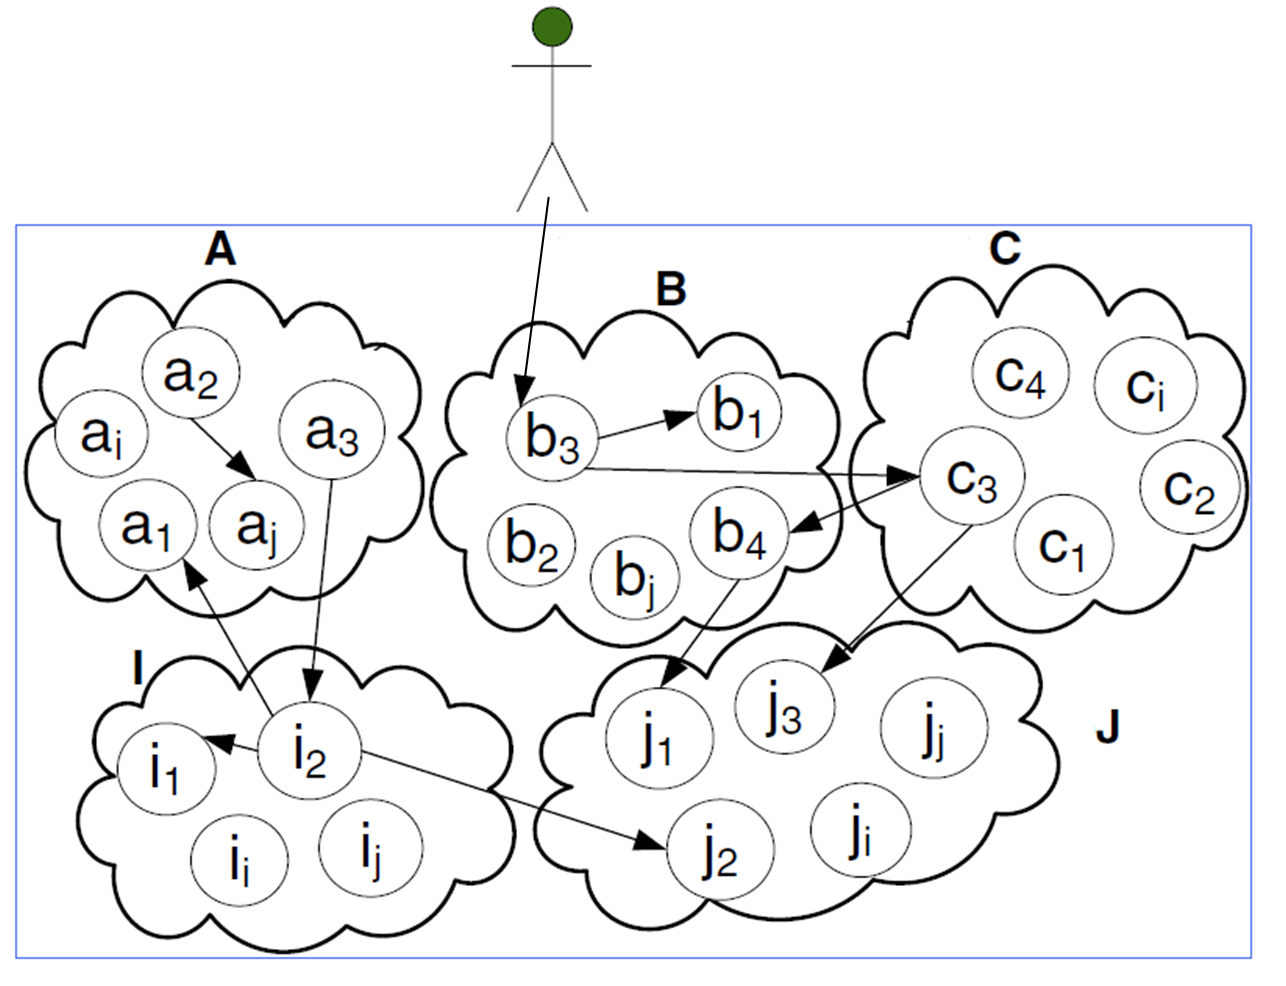
\includegraphics[width=.5\linewidth]{figures/choreography}}
    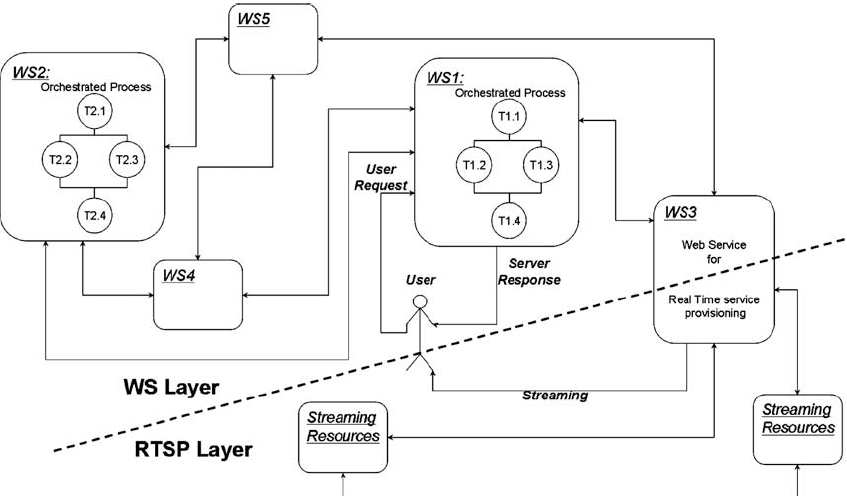
\includegraphics[width=.7\linewidth]{figures/choreography-scenario1.png}
    \caption{Choreography scenario about a CDN application\cite{Buccafurri2008a}}
    \label{figure:scenario}
\end{figure}


The SimGrid framework [3] is a simulation-based framework for evaluating cluster, grid and P2P mechanisms. SimGrid uses tasks to
 perform the simulation. Such tasks have an intrinsic cost to be transmitted over the network and an execution cost. Resources
 are described through an XML file in which it is possible to list available resources and their characteristics such as computing power, as well as available
links and routes to other resources. In another XML file the deployment of the simulated entities is described, ie,
where each simulated entity, also referred to as a Process, is deployed. Since the SimGrid allows the simulation of
distributed environments, we used it as the base to implement our simulator.


\subsection*{Execution environment}

Regarding the software,  
...

%Each service was deployed in a different node of the Open Cirrus
%testbed. Every node was running a 12.04 LTS 64 bit Ubuntu Linux, OpenJDK 6 and a custom installation of Apache Tomcat 7.0.25. 
%The only difference from the standard Tomcat configuration was the higher amount of maximum threads (from 200 to 1,024) in order 
%to handle more requests. The web services were developed using the Java API for XML Web Services (JAX-WS).

%Gus: Se for tratar como um experimento, o design precisa conter:
%- variavel independente e dependente
%- hipótese nula e alternativa
%...

\section*{Evidence the solution works}
The services were modeled as a set of working threads that receive a task sent over the network, execute it and then send
another task over the network to act as a web service response. The available methods and computational effort needed to
execute them, the amount of worker threads, medium size of the given responses, and service name are configurable through
a deployment XML file. And the choreography topology (host, communication channels  and links) is configured through
a platform XML file. Above this infrastructure, a monitoring is developed, and it's responsible of to measure the QoS attributes 
specified in table ~\ref{table:QoSmodel} of individual services  and to aggregate them in order to calculate global or composed QoS attributes
as total time response.




...
\section*{Competitive approaches}


Many simulators for distributed environments were proposed, eg., gridsim framework ~\cite{Buyya2002}, Pi4SOA [5], and SimGrid
framework [6]. The gridsim framework~\cite{Buyya2002} is a distributed environment simulation engine based upon on events. It implements entities
to emulate users. Users' requests are scheduled through a broker that allocates them into the simulated resources.
Pi4SOA [7] presents a policy-based infrastructure to dynamically verify and control the collaboration process in SOA. It is
also used as a starting point to develop an event driven policy enforcement in [8].

So, there is no simulations solutions for supporting service choreography enactment and even less with QoS support...

% \begin{figure}[ht]
% \begin{center}
% \includegraphics[height=0.5in]{techcon13_LaTeX_example_figure}
% \caption{The figure caption is below the figure.}
% \end{center}
% \end{figure}

\section*{Current status}
%N�s temos desenvolvido um simulador inicial  para realizar o ``enactment'' de coreografias, mas 
%para nossos objetivos adicionamos suporte de composi��o de QoS e infraestrutura de comunica��o.
We have developed a simulator to perform the `` initial'' enactment of choreography, but
our objectives for added support of QoS composition and communication infrastructure.

In this research project we are interested in the .... Our current efforts are
focused on the quantitative analysis. We are evaluating the
performance based on simulations, particularly interested in studying the effects of QoS composition on throughput
 of services and  networks aspects such as latency and bandwidth.

\section*{Next steps}


\tcreferences{
\bibliographystyle{abbrv}
\bibliography{references}
}

\end{document}
